\chapter{El Proyecto}

\section{Motivación}

En la actualidad existen pocos sistemas Aplicados en el ambito de la gestion en
el area de Medicina y los existentes suelen ser solo para areas especificas

\section{Descripci\'on del Proyecto}

INCOMPLETO



\section{Arquitectura de la Aplicacion}

Implementado en Python utilizando en Framework Django, utilizando el motor de bases
de datos PosgreSQL, funciona con una interfaz web por lo que se se accede al
mismo mediante un Navegador Web, Internamente maneja 2 Modulos principales
que son el  ``Modulo de Gestion de Turnos" y el ``Modulo de manejo de
Historia Clinica" , al ser un sistema web implementa un tercer modulo de manera
implicita que control de acceso mediante la definicion de Grupos Usuarios y
sus correspondientes permisos.

\section{Modulo Usuarios}

La gestion de usuarios es un proceso bastante comun en casi todos los sistemas,
muchos desarrolladores terminan programando funcionalidades de autenticacion 
una y otra ves a lo largo de los a\'nos y casi siempre funcionando de la misma 
manera. Django se penso para simplificar la vida no para complicarla, por eso
al ser una tarea bastante comun en casi todas las aplicaciones, viene incluido
un completo sistema de autenticacion que gestiona:

\begin{itemize}
    \item Usuarios
    \item Grupos
    \item Permisos
    \item Sessiones de Usuarios y Cookies
\end{itemize}

Aunque en cuanto a lo que se refiere manejo de sessiones es un completo sistema
solo maneja un peque\~no conjunto de datos por lo que hubo que estender mediante 
la adicion de un Modelo adicional para complementar la informacion de los 
usuarios.

\subsection{Modelos}

Aqui un diagrama con todos los modelos que componen el modulo Usuarios.

\begin{figure}[H]
    \centering
    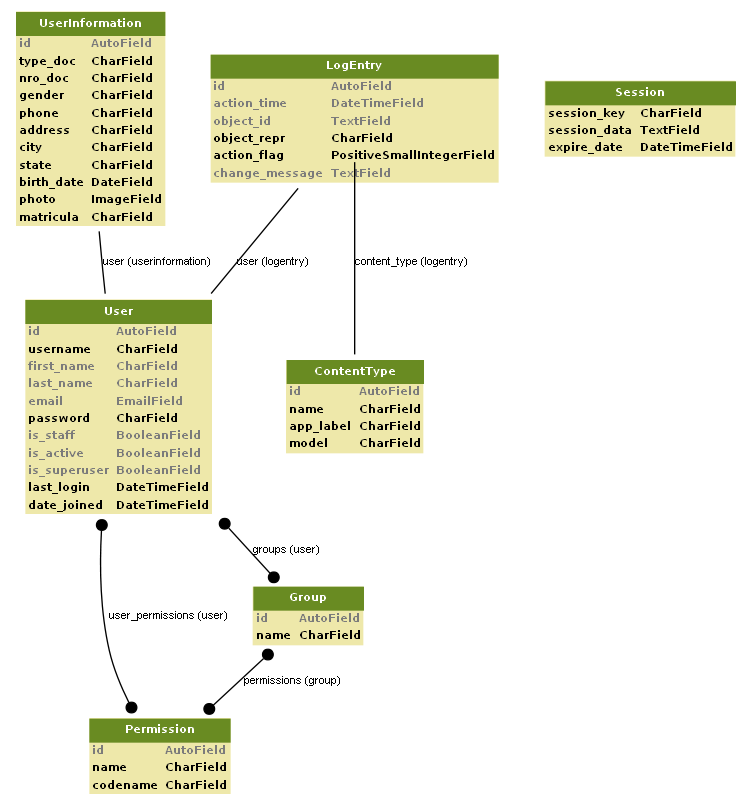
\includegraphics[scale=0.7]{resourse/auth.png}
    \caption{Diagrama con modelos que conponen el modulo Usuarios}
    \label{fig:07}
\end{figure}

Si lo expresaramos mediante la notacion UML para Diagramas de Clases 
tendriamos lo siguiente.

\begin{figure}[H]
    \centering
    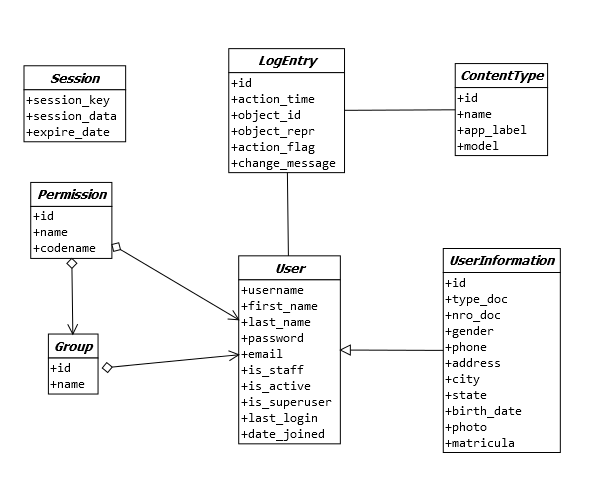
\includegraphics[scale=0.7]{resourse/uml-users.png}
    \caption{Diagrama con modelos que conponen el modulo Usuarios}
    \label{fig:07}
\end{figure}

El unico modelo que fue necesario agregar es UserInformation el resto vienen
con Django. En Resumen aunque se podria haber desarrollado Un Modulo desde
 cero que gestione las sessiones de usuarios hubiese generado trabajo extra sin
 sentido.

\section{Modulo Gestion de Turnos}

Dejando de lado el modulo Usuarios que nos provee Django el sistema desarrollado 
se divide esencialmente en 2 partes o modulos, aqui explicare como se dise\~no e
implemento el Modulo Gestion de Turnos, que a mi consideracion fue el que mayor
reto aporto a la hora de pensar un solucion para poder implementarlo.

El modulo se encarga de implementar las siguientes funciones

.Administracion de los datos de todos los Usuarios
.Asignacion de Turnos
.Mensajeria Interna



\section{Modulo Historia Clinica}

Este modulo del sistema tiene como tarea manejar y recolectar toda informacion 
referente a las historia clinica de los pacientes.

\subsection{?`Que es una Historia Clinica?}

Antes de entrar en todo lo referente sobre el desarrollo del correspondiente modulo
tomo un momento para explicar concretamente a que no referimos cuando hablamos de 
la misma por lo que aqui tenemos la siguiente definicion:

La historia cl\'{\i}nica es un documento m\'edico-legal que surge del contacto entre el 
profesional de la salud (m\'edico, pod\'ologo, psic\'ologo, asistente social, enfermero, 
kinesi\'ologo, odont\'ologo, etc.) y el paciente donde se recoge la informaci\'on necesaria 
para la correcta atenci\'on de los pacientes. La historia cl\'{\i}nica es un documento 
v\'alido desde el punto de vista cl\'{\i}nico y legal, que recoge informaci\'on de tipo 
asistencial, preventivo y social.

La Historia Clinica se origina con el primer episodio de enfermedad o control de salud en 
el que se atiende al paciente, ya sea en el hospital o en el centro de atenci\'on primaria, 
o en un consultorio m\'edico. La historia cl\'{\i}nica est\'a incluida dentro del campo de la 
semiolog\'{\i}a cl\'{\i}nica \footnote{La Semiolog\'{\i}a Clinica es el cuerpo del conocimiento
que se ocupa de la identificacion de las diversas manifestaciones patologicas 
\cite{SemiClin}}.

\subsection{La Historia Clinica en la Ley Argentina}

La documentaci\'on m\'edica comprendida en lo que com\'unmente se denomina ``historia 
cl\'{\i}nica" la cual no se encontraba regida por leyes especificas en la Argentina hasta
el 19 de noviembre del 2009 donde se promulga la Ley 26.529 \cite{LeyHC}.

En el cap\'{\i}tulo primero de la ley sen enumeran los derechos de los pacientes, 
en el art\'{\i}culo 2, inciso ``a". Renueva el derecho a la intimidad y la confidencialidad, 
donde se hace hincapi\'e sobre la responsabilidad de preservar la intimidad y 
confidencialidad de toda la documentaci\'on m\'edica concerniente a los pacientes, 
particularmente el inciso ``d" del mismo art\'{\i}culo:

``El paciente tiene derecho a que toda persona que participe en la elaboraci\'on 
o manipulaci\'on de la documentaci\'on cl\'{\i}nica, o bien tenga acceso al contenido de 
la misma, guarde la debida reserva, salvo expresa disposici\'on en contrario 
emanada de autoridad judicial competente o autorizaci\'on del propio paciente"

Garantiza adem\'as el respeto por la autonom\'{\i}a del paciente y el derecho a recibir 
la informaci\'on necesaria para su salud, incluyendo el derecho a negarse a ser 
informado.

El cap\'{\i}tulo III reza sobre el Consentimiento Informado, el cual est\'a basado en 
el principio de autonom\'{\i}a, es decir, el derecho del paciente a ser reconocido 
como persona libre y due\~na de tomar sus decisiones. Para ello el paciente debe estar en 
condiciones de comunicar su decisi\'on y  \'este ha sido informado adecuadamente de 
sus opciones, es decir, no pueden ser decisiones hechas como resultado de delirio 
o alucinaciones. La decisi\'on del paciente es consistente con sus valores y metas 
y se mantiene estable en el tiempo si no han habido modificaciones hechas por
el mismo sujeto. Los familiares de un paciente no est\'an en el derecho de 
requerir al m\'edico del paciente que no se le comunique ciertos detalles o
informaci\'on al mismo. 

Ahora bien vallamos a lo que nos interesa:

La ley define a la Historia Cl\'{\i}nica como el documento ``obligatorio, cronol\'ogico,
foliado y completo en el que consta toda actuaci\'on realizada al paciente por
profesionales y auxiliares de la salud." Define que la historia cl\'{\i}nica es 
propiedad del paciente, siendo este el titular de la misma. Siempre que un paciente 
solicite la historia cl\'{\i}nica, la instituci\'on competente debe entregarle una copia
autenticada en 48 horas. Si no es entregada en ese plazo, el
paciente est\'a autorizado a interponer un recurso de Habeas Data, juzgado de por 
medio. 

Entre los datos que han de consignarse en forma obligatoria esta la fecha de 
inicio y confecci\'on de la historia cl\'{\i}nica, datos identificatorios del paciente
y su n\'ucleo familiar, datos del profesional interviniente y su especialidad, 
registros claros y precisos de los actos realizados por profesionales y auxiliares
intervinientes, antecedentes gen\'eticos, fisiol\'ogicos y patol\'ogicos si los hubiere,
y todo acto m\'edico realizado o indicado.

Incluye en la historia cl\'{\i}nica a todos los documentos que hagan referencia a 
informaci\'on de salud del paciente, a\~nadiendo los consentimientos informados, 
hojas de indicaciones, hojas de enfermer\'{\i}a, estudios complementarios, 
incluyendo las``pr\'acticas realizadas, rechazadas o abandonadas." 
Esto  \'ultimo es interesante: si el paciente abandona o rechaza un tratamiento 
propuesto, es responsabilidad del m\'edico consignarlo, que a fin de cuentas es el
beneficiario de que aquello quede asentado desde el punto de vista m\'edico-legal.

Autoriza a reclamar una copia de la historia cl\'{\i}nica al paciente y su representante 
legal, al c\'onyuge o conviviente de hecho (sin importar el sexo), y a los herederos 
forzosos. Lo que no queda claro del art. 19 inciso b es si los c\'onyuges y 
convivientes requieren o no la autorizaci\'on del paciente.

Se a\~nade esta ley al cap\'{\i}tulo 11 del C\'odigo de Etica de la Asociaci\'on M\'edica 
Argentina, del a\~no 2001. En ella se explaya en forma m\'as extensa y detallada sobre
la confecci\'on. Particular inter\'es debi\'eramos prestarle al art. 168:

``La historia cl\'{\i}nica ha de ser un instrumento objetivo y comprensible por terceros,
y no solo por quienes escriben en ella." A su vez, el art. 171 especifica que 
"debe ser legible, no debe tener tachaduras, no se debe escribir sobre lo ya 
escrito, no debe ser borrada, no se debe dejar espacios en blanco y ante una
equivocaci\'on debe escribirse ERROR y aclarar lo que sea necesario. No se debe a\~nadir
nada entre renglones."


\subsection{Funcionalidades}

Las funcionalidades que se implementan en correspondiente modulos son solo
basicas y comprenden la documentacion practicas mas comunes dentro del area de la 
medicina, esto no implica que solo valla a servir para eso unicamente, por su 
extructura el modulo contempla la posibilidad de agregar nuevos componentes para 
estudios especificos que sean requeridos y que no hayan sido contemplados en el 
actual sistema.







\section{Elecci\'on de la metodolog\'ia de Programaci\'on}

